%
% plane.tex -- Bild der Fluzeuge
%
% (c) 2019 Prof Dr Andreas Müller, Hochschule Rapperswil
%
\documentclass[tikz,12pt]{standalone}
\usepackage{amsmath}
\usepackage{times}
\usepackage{txfonts}
\usepackage{pgfplots}
\usepackage{csvsimple}
\usetikzlibrary{arrows,intersections,math}
\begin{document}

\newboolean{showgrid}
\setboolean{showgrid}{false}
\def\breite{3}
\def\hoehe{3}

\begin{tikzpicture}[>=latex,thick]

\begin{scope}[xshift=-4.2cm]
\node at (0,0) {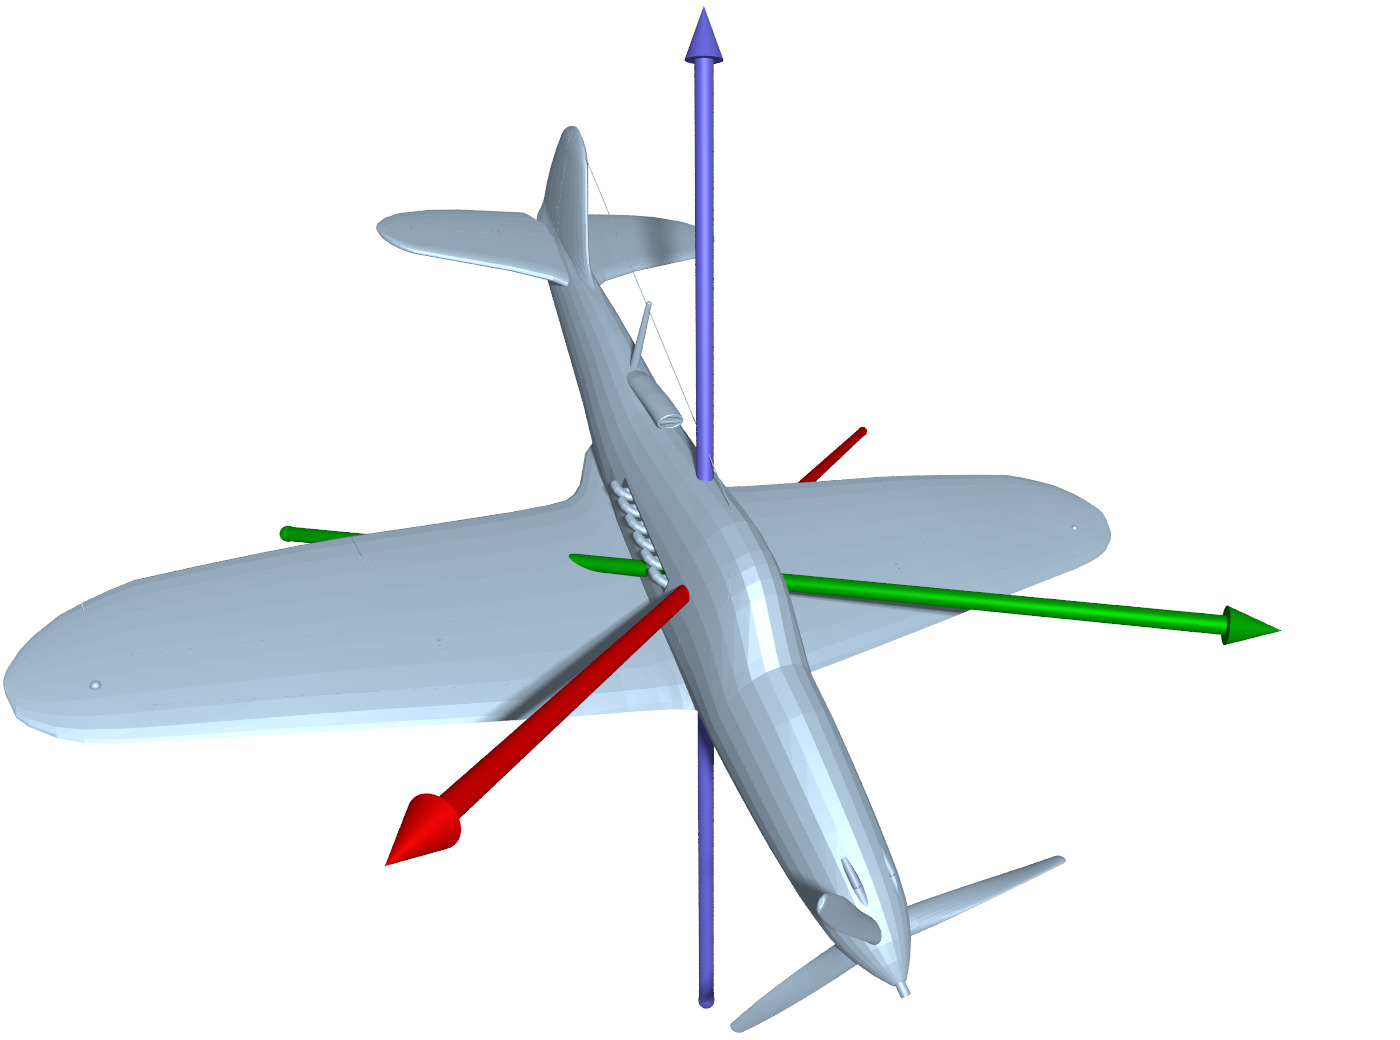
\includegraphics[width=8.0cm]{../60000035/plane2.jpg}};
\ifthenelse{\boolean{showgrid}}{
\draw[step=0.1,line width=0.1pt] (-\breite,-\hoehe) grid (\breite, \hoehe);
\draw[step=0.5,line width=0.4pt] (-\breite,-\hoehe) grid (\breite, \hoehe);
\draw                            (-\breite,-\hoehe) grid (\breite, \hoehe);
\fill (0,0) circle[radius=0.05];
}{}
\node at (-2.0,-1.8) {$x$};
\node at (3.2,-0.3) {$y$};
\node at (0.3,2.8) {$z$};
\end{scope}

\begin{scope}[xshift=4.2cm]
\node at (0,0) {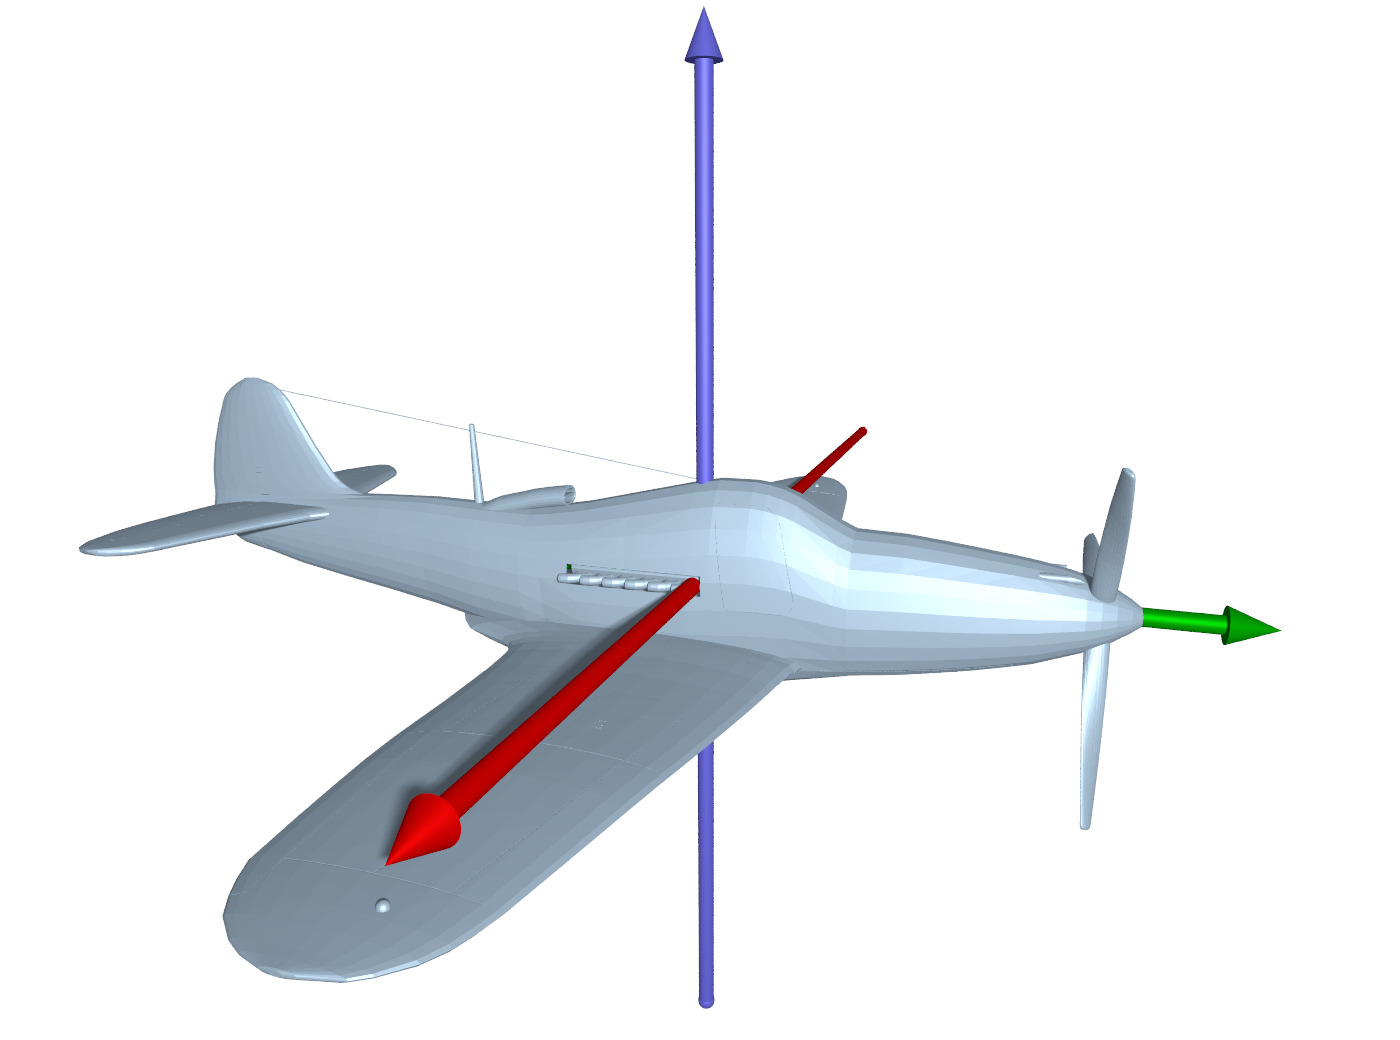
\includegraphics[width=8.0cm]{../60000035/plane3.jpg}};
\ifthenelse{\boolean{showgrid}}{
\draw[step=0.1,line width=0.1pt] (-\breite,-\hoehe) grid (\breite, \hoehe);
\draw[step=0.5,line width=0.4pt] (-\breite,-\hoehe) grid (\breite, \hoehe);
\draw                            (-\breite,-\hoehe) grid (\breite, \hoehe);
\fill (0,0) circle[radius=0.05];
}{}
\node at (-2.0,-1.8) {$x$};
\node at (3.2,-0.3) {$y$};
\node at (0.3,2.8) {$z$};
\end{scope}

\end{tikzpicture}
\end{document}
